%\documentclass[11pt]{article}
\documentclass{llncs}
\usepackage[latin1,utf8x]{inputenc}
\usepackage{color}
\usepackage[pdftex]{graphicx}
%\usepackage{amsmath, amsfonts, amssymb, amsthm}
\usepackage{amsmath}


\title{Titolo da decidere}
\author{authors}
\date{date}
\begin{document}
\maketitle
\begin{abstract}
This is a very short abstract.
\end{abstract}

\section{Introduction}

Process mining is a recent discipline that includes techniques for process analysis and discovery. Today, many Information Systems that integrate the concept of business process provide registration of events that occur during the process activities. Starting from recorded executions related to the same process, the goal of the process mining techniques is extracting data to discover automatically a process model or, if the model already exists, to check the executions in term of conformance and performance.\\

The idea of this work consists in developing an approach for exploiting the huge ammount of data recorded in the process activities by the information systems. More precisely, our purpose is to find pattern on data that could influence the process behaviour. For this reason, the work presented in this paper is based on some concepts of Machine Learning and Data Mining. Should be noted that using data mining for similar aims has already been explored by Van der Aalst in \cite{}, the idea there consists in discovering how data attributes may influence the routing of cases. Instead, in this contribution the intention is to present an approach based on data mining techniques also, but for discovering dependencies between process data and its conformance and performance. Finally, another goal that we pursue is providing a predective model to check the conformance result and some performance metrics for the future process executions.  \\

%In front of a very large number of process instances, all recorded in event log, it is essential to have an automatic tool for extracting usefull information for the analysis of the real behaviour of the process. In order to meet this requirement, in this article we present an approach based on classification and decision trees to identify rules that could influence the process in term of conformance to the existing model, and performance metrics.\\
%\newline
%\textcolor{blue}{
%}

%Il process mining comprende una serie di tecniche che trattano processi vigenti in contesti organizzativi. Attualmente, moltissimi sistemi che integrano il concetto di processo di business a loro interno, provvedono alla registrazione degli eventi che si verificano durante l'esecuzione delle attività previste dal processo. Partendo da un insieme di esecuzioni registrate e riguardanti un unico processo, è possibile applicare una serie di tecniche volte alla scoperta del modello di processo oppure alla sua analisi in termini di conformance e performance. L'idea che ispira questo articolo è sviluppare un approccio in grado di sfruttare le enormi quantità di dati che vengono registrati in corrispondenza delle varie attività del processo.
%Si tratta di un approccio basato sulle tecniche di data mining capace di scoprire eventuali influenze dei dati sul comportamento del processo. L'impiego del data mining per il process mining è un'idea già presentata da Van deer Aalst in \cite{}, in questo articolo infatti si cerca di evidenziare le influenze dei dati sulla direzione del flusso di esecuzione in corrispondenza dei punti decisionali. La nostra idea invece è di sfruttare le tecniche di data mining per fornire agli analisti di porcesso un tool di supporto in grado di aiutare nell'analisi di conformance e performance del processo.\\




%Di fronte ad un numero molto grande di istanze di processo, tutte appositamente registrate in event log, avere uno strumento capace di estrarre informazioni utili per l'analisi del comportamento reale del processo diventa fondamentale. Cercando di rispondere a questa esigenza, in questo articolo è presentato un approccio capace di individuare eventuali regole che influenzano il processo in termini di conformance al modello prefissato, ed in termini di performance. Un ulteriore obiettivo che ci poniamo è fornire agli analisti uno strumento di predizione, ovvero un modello in grado di predire, in base ai dati delle nuove istanze di processo che si presentano, quale sarà l'esito di conformance e le misure di performance che caratterizzano la particolare esecuzione presa in esame. Per potere realizzare questi obiettivi ci basiamo sulla classificazione che è una particolare tecnica di data mining, vengono inoltre impiegati gli alberi di decisione come strumento di classificazione.\\


%L'articolo è organizzato in questo modo: dopo una presentazione nella sezione 2 dei vari formalismi adottati, nella sezione 3 viene presentato un semplice esempio a cui verrà fatto riferimento nell'articolo. Nella sezione 4 invece verranno introdotti alcuni concetti relativi alla conformance e performance di un processo. Infine, nella sezioni 5 e 6 si affronterà come impiegare la tecnica di classificazione per scoprire particolari pattern nei dati che possono influenzare conformance e performance del processo.


%The article is organized as follows. After an introduction to the different formalism used to carry out our purposes, the attention will be...


\section{Example}\label{example}
To clarify what presented in this paper the example illustrated in this section will be taken into exam whenever is needed.\\

Commercial organizations usually follow a specific procedure to manage orders received from various clients. In general this procedure represents a business process that includes many different activities, each of them can involve diffent departments of the organization. Let us consider a semplification of this procedure. For us, the sale process begins with receving an order notification from a client, so the first process activity is simply called ``Order''. After the order is received the sale process continues with some activities that can be done in parallel (since they do not present any dependencies). One of these is the ``FinancialCheck'' activity during which the order is analysed from a financial point of view (for example verifying the client situation and solvency). In parallel an activity called ``WarehouseCheck'' is performed. In this phase a check regarding the merchandise requested by the order is done, and in case of a shortage an external order is issued for a supplying, this is done through the activity ``ExternalWarehouse''. After the completion of the  parallel activities, a synchronization is needed before continuing the sale procedure. In the semplification considered here the sale process terminates with the activity ``Notify'' in which a result regarding the acceptance of the order is comunicated to the client.\\

There are many differents formalisms for modeling business processes, the most popolar are based on flowcharts because of their expressivness (BPMN for instance). For our purposes, a process is represented by a Petri net which is a mathematical model characterized by rigor and suitable for process mining analysis. It is worth noting that there exist some techniques that allow transforming a model expressed in a flowchart to a model expressed with a Petri net, more information can be found in \cite{}. The petri net representing the sale process discussed in this section is shown in figure \ref{pnet}. The Petri net is obtained by transforming a BPMN model in which each activity can have only tow possibile state: start state, denoting the begin of the activity, and the end state.

\begin{figure}[h]
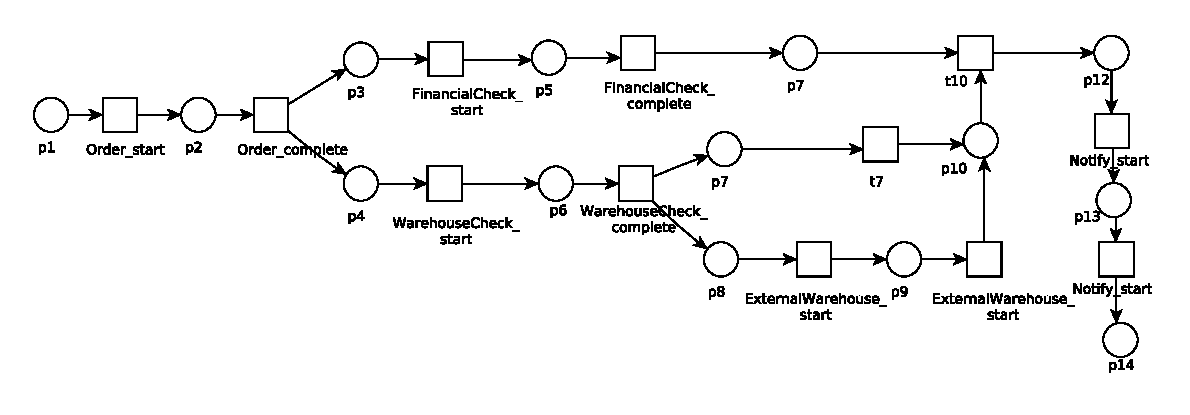
\includegraphics[width=360pt]
{./items/Sales_PN.pdf}
\caption{Petri net}
\label{pnet}
\end{figure}


\section{Process Analysis}\label{Background}

The process analysis is performed by using the Petri net modeling the process and an event log recording the related executions (process instances). The basic building blocks of event logs are events. An event {\itshape e} can be seen as a pair {\itshape e = (a,t) } representing an action {\itshape a } recorded and the corresonding timestamp {\itshape t}. Action and timestamp are denoted respectively by $\alpha(e)$ and $\phi(e)$. Events that belong to the same process are grouped into {\itshape traces}. Formally, a trace $T$ is a finite sequence of events $T[1],..., T[n]$, such that $\phi(T[i]) \leq \phi(T[i+1])$ for all  $i \in [1,n)$. A log $L$ is a set of traces, recording the activities performed by a system during a finite number of process executions. We assume here the following hypothesis:
\begin{itemize}
\item All traces are instances of the same process.
\item For each action there exists a corresponding transition in the net that will be denoted, for simplicity, by the same name of the action.
\end{itemize}

\subsection{Log replay algorithm}

The key algorithm expoloited to analyze the Petri net model with respect to the log is the {\itshape log replay} algorithm \cite{} .Given a Petri net model and an event log as intput to the algorithm, the output results can be used to check the conformance of traces and to evaluate some performance metrics. For each trace in the log, log replay starts by placing one token in the start place of the net. For each event in the trace the corresponding transition is fires in an {\itshape non blockin way} and the marking of the net is updated. ``Non blocking replay'' means that if the log replay execution requires to fire an enabled transition, the missing tokens are created artificially. The output of the log replay of a trace can be represented as an orderd list $R$ of pairs $(tr, i)$, representing that the transition $tr$ has been fired to mimic the event $T[i]$.
\\

In general, there could exist some transition in the net called {\itshape invisible}. This can happen if the transition models an internal choice that is not visible in the system, or it is used to implement a construct of a more abstract modelling language (BPMN or others). Usually, invisible transitions are considered to be lazy, i.e, when firing a visible transition $t$ corrisponding to an event of the trace is needed, only then the invisibile transition enabling $t$ is fired. However, in this paper, we adopt an other way for handling these transitions: the firing is performed as soon as possible. This allows to carry out some performance measures   that are not possible with the lazy methode as explained in \cite.(riferimento al paper Applying Process Analysis to the italian eGov Entreprise Architecture)\\

The result of log repaly can be used to evaluate conformance and performance of the Petri net model. Conformance problems can be discovered by analyzing the tokens that have been artificially created {\itshape (the missing tokens)} and the tokens that were not consumed {\itshape (the remaining tokens)}.\\

\subsection{Conformance Analysis}
To clarify the conformance analysis technique we exploit the Petri net presented in section \ref{example} with reference to tow traces, $T$ and $T'$, presented respectively in figures \ref{ConfLog} and \ref{NonConfLog}. The log replay execution of the trace $T$, which is compliant with the Petri net, terminates with a marking containing one token in the end place \{${p14 \rightarrow 1}$\}, and returns the sequence:
\begin{equation}
\begin{split}
R&=\{(Order\_start,1), (Order\_complete,2),(WarehouseCheck\_start,3), \\
& (FinancialCheck\_start,4),(FinancialCheck\_complete,5),\\
& (WarehouseCheck\_complete,6),(t5,7),(t7,7),(t10, 7), (Notify\_start,7), (Notify\_complete,8)\}
\end{split}
\end{equation}


The log replay execution of the trace $T'$ terminates with remaing tokens \{${p8 \rightarrow 1,p14 \rightarrow 1}$\} and a missing token \{${p10 \rightarrow 1}$\}. The missing token is created artificially and this fact records a wrong execution of the event $Notify\_start$. In fact, notice that in the trace $T'$ this event is executed before the termination of the activity ``FinancialCheck'', and this is interpreted as a non conformance to the process model. The sequence returned by log replay is:
\begin{equation}
\begin{split}
R'&=\{(Order\_start,1), (Order\_complete,2), (WarehouseCheck\_start,3), \\
& (FinancialCheck\_start,4), (WarehouseCheck\_complete,5),(t5,6),(t7,6), (t10,6)\\
& (Notify\_start,6), (Notify\_complete,7)\}
\end{split}
\end{equation}

\begin{figure}[t]
\centering
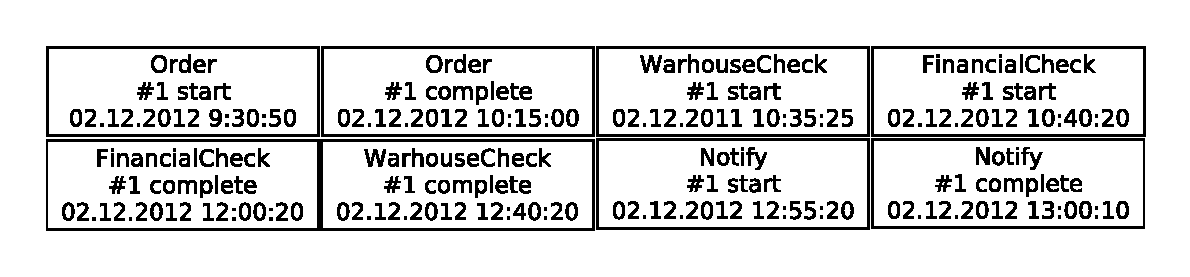
\includegraphics[width=400pt,height=40pt]
{./items/logConforme.pdf}
\caption{Conforme log example}
\label{ConfLog}
\end{figure}

\begin{figure}[h]
\centering
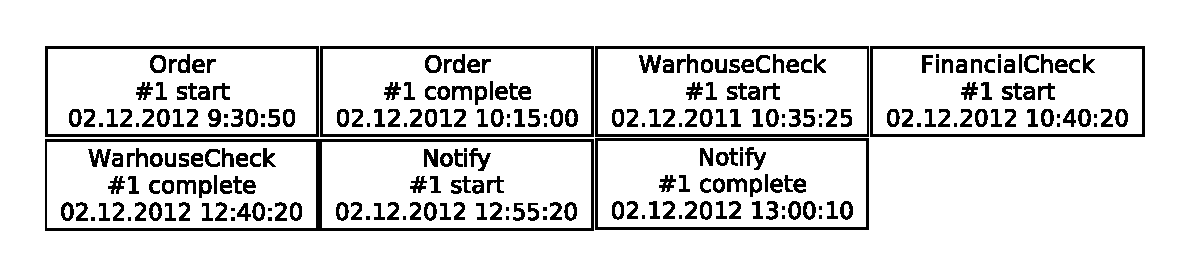
\includegraphics[width=400pt,height=40pt]
{./items/logNonConforme.pdf}
\caption{Non conforme log example}
\label{NonConfLog}
\end{figure}

\subsection{Performance analysis}
A performance analysis of a process can also be done based on the log replay results. Since the logs contain timestamps, the log replay can be used to compute performance measures of the process. The idea is to calculate the time interval between production and consumption of tokens in each place. Analysing performance can be applied only to traces that do not present missing token during the replay, because such tokens cannot have time information. During the log replay the following metrics can be computed for each trace and each place:
\begin{itemize}
\item sejour time $(tsj)$ : the time interval between arrival and depature of tokens;
\item synchronization time $(tsc)$: the time interval between arrival of a token in the place and enabling of a transition in the post-set of the place;
\item waiting time $(tw)$:  the time interval between enabling of a transition in the post-set of the place and token departure (thus $tsj=tsc+tw $).
\end{itemize}

To clarify the metrics evaluated by this tecnique, as done with conformance analysis, we exploit the Petri net  presented in section \ref{example} and the trace T presented in figure \ref{ConfLog}. The replay starts with firing the transition $Order\_start$ at time $0s$, thus a token arrives at $p2$ at time $0s$. After $45 min$ the token in $p2$ is consumed and the transition $Order\_complete$ is fired, so $tw(p2)=45min$, and a token arrives at $p3$ and $p4$. At the time $1h:5min:25s$ the transition $WarhouseCheck\_start$ is fired, thus $tw(p4)=20min+25sec$ and a token is produced at $p6$. At the time $1h:10min:20s$ the transition $FinancialCheck\_start$ is fired and a token is produced at $p5$, so $tw(p3)=25min+20s$. After $2h:30min:20s$ from the replay start the transition $Financial\_complete$ is fired, hence we have $tw(p5)=1h+20min$ and a token is produced at $p11$. At time $3h:10min:20s$ the firing of the transition $WarehouseCheck\_complete$ is executed, so $tw(p6)=2h+4min+55s$ and token is produced at $p7$. After $15 min$ the invisible transition $t7$ is fired and a token is produced at $p10$. At this point the transition $t10$ is enabled, so firing it is now possible and a token is produced at $p12$. Notice that $tsc(p11)=40min, tsc(p10)=0s$. At the time $3h:25min:20s$ the transition $Notify\_start$ is fired and a token is produced in $p13$, after $4min+4sec$ the transition $Notify\_complete$ is fired and $tw(p13) = 4min+40s$.\\

An important performance measure is the activity execution time. This can be deducted from the waiting time in the places between the start and the complete transitions of each activity. For example, time execution for ``FinancialCheck'' is given by the waiting time computed for the place $p5: tw(p5)=1h+20min$.\\

It is worth noting that the synchronization time is greater than zero only for places which contain on their post-set transitions depending from other places. For the Petri net in figure \ref{pnet}, the only places which can have a synchronization time not null are $p10$ and $p11$. For instance, the sycronization time is greater than zero for $p11$ in the trace in figure \ref{ConfLog}. That means that, for this particular instance of the process, the branch with the activity related to the Financial checking is faster than the branch with the warehouse activities.

\section{An approach based on classification for Process Analysis}\label{ClassConformance}
%Supponiamo di avere un numero altissimo di esecuzioni relative al medesimo processo registrate in event log. Supponiamo anche che tutte queste esecuzioni siano state analizzate dal punto di vista della conformance per mezzo del log replay. L'algoritmo di analisi log replay si limita ad individuare come mostrato in sezione \ref{Background} quali sono i punti in cui si verificano errori di conformance, tuttavia, esso non fornisce alcuna informazione sulle cause che generano queste anomalie.\\

%Riuscire ad individuare anomalie è uno degli obiettivo fondamentali nell'analisi dei processi, avere un'idea su quali sono le cause che li generano lo è ancora di più. Questo infatti permette di capire anche come agire per apportare eventuali correzioni. 
 
%Perciò l'idea che ci ha guidato in questo lavoro consiste nel riuscire ad individuare nei dati contenuti negli event log, eventuali pattern che possono influenzare gli scostamenti rispetto al modello prestabilito. Questo infatti potrebbe aiutare nell'individuare le cause che stanno dietro agli scostamenti del comportamento reale del processo rispetto a quello atteso.

Employing data mining techniques for process analysis was already experimented by Van Deer Aalst in \cite{decision mining in business process}. In that paper the idea consists in discovering how data attributes may influence the routing of cases. This work is motivated by the presence of a huge ammount of data recorded in the event logs in the form of attributes that could contain implicit information. In this contribution, the same methodology is adopted to offer an additional tool for process analysis.\\

With the approach presented here, our goal is to discover patterns or rules in the event logs data in corrispondence of which conformance errors, discussed in section \ref{Background}, occur. The goal is to conduct an investigation into data to discover the cause of conformance anomalies. Given the enormous quantity of data, the analysis is carried out with \emph{classification}, a classical data mining technique.


\subsection{Classification: basic concepts}

In a classification problem, data is represented by a collection of records (called instances), each of them is characterized by a tuple $(\mathbf{x},y)$, where $\mathbf{x}$ is an attribute set, while $y$ is a special attribute called ``target attribute'' denoting the class to which the record belongs. With this technique, the idea is learning a classification model that maps each attribute set $x$ to one of the predefined class labels $y$.\\

A classification model is useful for the following purposes:
\begin{itemize}
\item Descriptive Modeling: A calssification model can serve as an explanatory tool to distinguish between objects of different classes.
\item Predictive Modeling:  A classification model can also be used to predict the class label of unknown records. In fact, a classification model can be treated as a black box that automatically assigns a class label when presented with an attribute set of an unknown record.
\end{itemize}

Many classification models could be used for a classification problem. For our purpose we choose the decision tree model because of its simplicity and diffusion. In a decision tree, to each leaf node is assigned a class label (a possible value of the attribute target). The non-terminal nodes, which include the root and other internal nodes, contain attribute test conditions to separate records that have different characteristics. In principle, there are exponentially many decision trees that can be constructed from a given set of attributes. While some of the trees are more accurate than others, finding the optimal tree is computationally infeasible because of the exponential size of the search space. However, efficient algoritms have been developed to induce a reasonably accurate decision tree in a reasonable amount of time. These algorithms usually employ a greedy strategy that grows a decision tree by making a series of decisions about which attribute to use for partioning the data. For instance Hunt's algorithm is one of theme and it represents the basis of many existing decision tree induction algorithms, including $C4.5$ algorithm used for our purposes.\\
See \cite{} for more information about classification.\\


\subsection{Classification for Conformance Checking}
Analysing data arising from event logs can be transformed into a classification problem. The data set can be derived from the process data, In particular, each instance data determines a record of the data set. For the process presented in section \ref{example}, a record is charaterized by the following attributes set: an instance identifier, a client identifier, the client typology with two possible values: new client and consolidated client, the sales manager responsabile for the order, the chief financial officier name who conducts the financial evaluation activities, the warehouseman name for the warehouse check activities, a supplier name in case of an external warehouse activity, and finally the result communicated to the client for the order issued. The conformance result for the process instance provides an additional and important data which takes the role of the target attribute. All these attributes are discrete and contribute to formulate the data set presented in table \ref{tab:SaleData} of the classification problem.\\

\begin{table}[!h]
\scriptsize
\centering
\begin{tabular}{|p{1cm}|p{1cm}|p{1,5cm}|p{1,2cm}|p{1,4cm}|p{1,2cm}|p{1cm}|p{1,4cm}|p{0,8cm}|}
\hline OrdIde & CltIde & CltType & SalMan & FinOff & WrhsMan & Supplier & OrdResut & Conf\\
\hline
1 & 20 & consolidate & Marco & Alessandro & Alex & Gianni & positive & yes\\
\hline
2 & 15 & new & Anna & Mario & Alessio & Mario & positive & yes\\
\hline
3 & 10 &consolidate & Maria & Roberto & Alessio & Gianni & negative & yes\\
\hline
... & ... & ... & ... & ... & ... & ... & .... & .... \\
\hline
... & ... & ... & ... & ... & ... & ... & .... & ...  \\
\hline
\end{tabular}
\scriptsize
\caption{Data set}
\label{tab:SaleData}
\end{table}
\normalsize

Using existing data mining tools for classification, it is possible to build a decistion tree as a classification model for the example presented here. We do this based on data produced artificially just for exemplary purposes: from the event log recorded, the attributes that characterize the process are extracted, and all the resources needed for the classification algorithm employed are produced. The resulting decision tree is presented in figure \ref{salesDecTree}.\\

\begin{figure}[h]
\centering
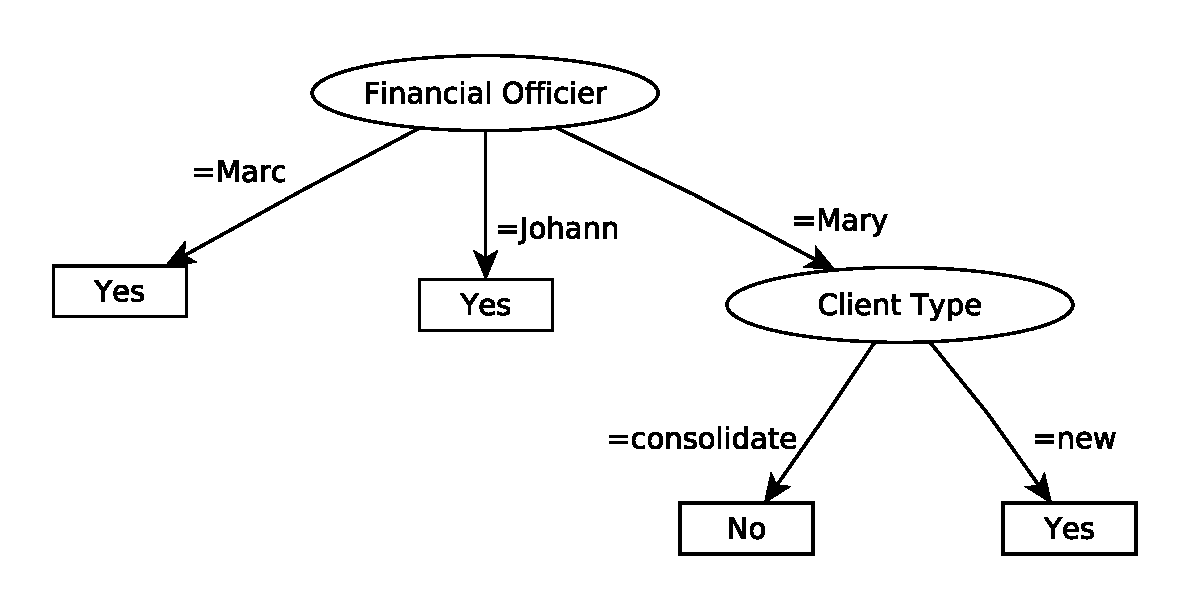
\includegraphics[width=230pt,height=110pt]
{./items/Sales_tree.pdf}
\caption{decision tree}
\label{salesDecTree}
\end{figure}
The decision tree returned describes a data pattern in correspondence of which a process instance could present conformance errors: order managed by the sales manager ``Mary'' and received from consolidate clients of the organization may not respect the standard sales procedure. However, to get information most significant for our analysis, it is useful to relate what is noticed by the decision tree with the log replay results. In figure \ref{replayResult} is presented a Petri net that resumes the conformance analysis conducted on instances recorded in the event log taken in exam. Arcs are labled by the number of activations done. Places, whenever presents some remaining or missing tokens, are labled by the number of these tokens.\\
\begin{figure}[h]
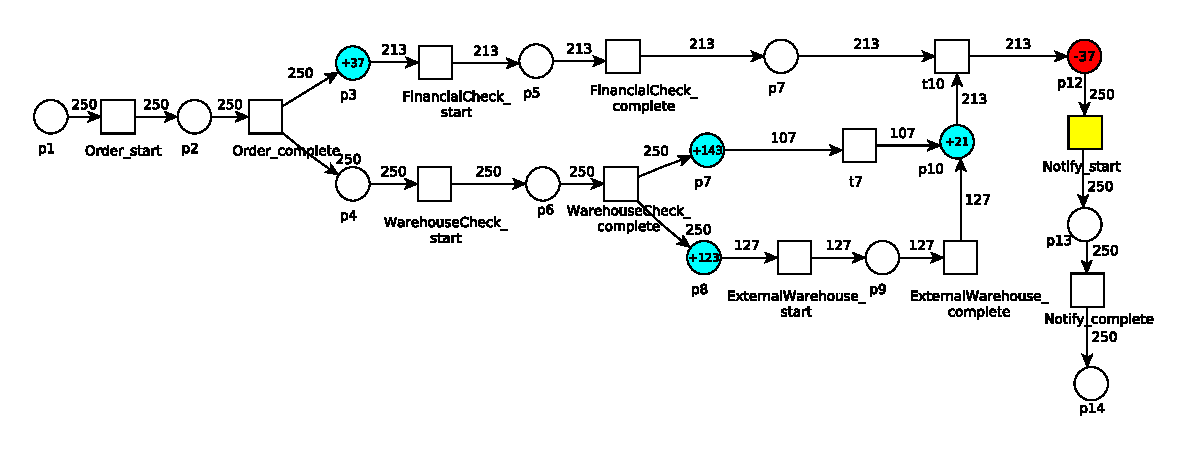
\includegraphics[width=390pt]
{./items/Sales_PN_result.pdf}
\caption{Petri net}
\label{replayResult}
\end{figure}

The Petri net reporting the log replay results shows that there are 37 of 250 process executions with conformance erros. In fact, the presence of 37 missing tokens in $p12$ signals a forced execution of the transition ``Notify\_start''. In order to give an interpretation for this results, it must be taken into account the non blocking behaviour of the log replay. In this case, the 37 missing tokens in $p12$ notice that during the replay the algorithm needs to mimic the event ``Notify\_start'' but the transition associated to the event is not enabled in the marking reached by the net, so the algorithm creates artificial tokens for completing the trace replay. This situation is possible only if the invisible transition $t10$ is not enabled. Now, if $t10$ is not enabled that means that there are no tokens in the place $p10$ or $p7$. But notice that there are 21 remaining tokens in the place $p10$, so the transition $t10$ is not enabled for those $37$ instances because the place $p7$ does not present tokens. Moreover, the Petri net in figure highlights 37 remaing tokens in the place $p3$, so we can deduce that in those instances financial activities were not performed. From this facts, we can conclude that the conformance problems presented in  37 instances are due to a missing execution of the financial activities check. On the other hand, the decision tree reports that the instances with conformance problems are made by consolidate clients. In this case, it might be reasonable that, for the orders made by the consolidate clients of the organization, could not be necessary a financial valutation of their situation.\\


The analysis based on a combination of the log replay results and the pattern data described by the classification, may allow to discover new cases of the business procedure to take into consideration during a possible process extension. For instance, with the analysis done before, in order to extend the model presented in section \ref{example} we can include what it was discovered: for the orders done by the consolidate clients of  the organization, the financial check activity is not needed. In other cases, whenever  a process extension is not possible (i.e. a fixed procedure to be strictly respected), such kind of analysis can help in taking corrective measures in order to avoid conformance errors. In particular, through a combination of the log replay results and the data patterns rules it may be possible to discover (and localize) conformance errors causes. This fact can be fundamental to bring the right corrections. For instance, in our sale process, if the procedure described by the model must be respected in any case, a revision on the staff behaviour about consolidate clients can be done in order to avoid conformance errors.\\

The classifier constructed with this approach can be used not only in a descriptive sense but also in predictive way. In fact, given a new event log, in order to perform the conformance checking to the process model, the decision tree obtained can be used to predict the conformance result of the new process instances. This can allow some advantage in term of the execution time since the log replay algorithm can take more time than the one needed by a decision tree to classify a new instance. Also, it is worth noting that, whenever the set of attributes needed for classification is known before the execution of the process instance, it can be interesting to predict the conformance result of the instance and avoid the errors that could happen during the execution.




\subsection{Classification for Perfomance Analysis}\label{ClassPerf}

The approach presented in section \ref{ClassConformance} can be extended for performance analysis. Using classification technique for discovering how data attribute can influence process performance provides useful information in analysing and optimizing the process services. For example, discovering data patterns in correspondence of which some activities need more time for completion than others, helps in making decision about resources distribution to various process activities or in scheduling activities.\\

In addition to the execution or completion time, classification can be used to discover information about more complex performance metrics such as the syncronization time. Processes with parallel activities and syncronizations can often present activities that represent a bottleneck, this leads to increase the waiting time of some activities and consequently the completion time of the entire process. In this context, with the approach presented in this paper, the goal is to discover rules in the process data that influence the syncronization time. The model built by classification techinque can be used also in a predicting way, and this is certainly very important in order to optimize performance execution of the process.\\

\begin{table}[!h]
\scriptsize
\centering
\begin{tabular}{|p{1cm}|p{1cm}|p{1,5cm}|p{1cm}|p{1,3cm}|p{1,4cm}|p{1,1cm}|p{1,2cm}|p{1,5cm}|}
\hline OrdIde & CltIde & CltType & SalMan & FinOff & WrhsMan & Supplier & OrdResut & Synch\\
\hline
1 & 20 & consolidate & Marco & Alessandro & Alex & Gianni & positive & high\_wareh.\\
\hline
2 & 15 & new & Anna & Mario & Alessio & Mario & positive & normal\\
\hline
3 & 10 &consolidate & Maria & Roberto & Alessio & Mario & negative & normal\\
\hline
2 & 15 & new & Anna & Mario & Roberto & Gianni & positive & high\_wareh.\\
\hline
... & ... & ... & ... & ... & ... & ... & .... & .... \\
\hline
... & ... & ... & ... & ... & ... & ... & .... & ...  \\
\hline
\end{tabular}
\caption{Data set}
\label{tab:SaleDataPerf}
\end{table}
\normalsize

With reference to the example in section \ref{example} and to the performance metrics explained in section \ref{Background}, in this paragraph the approach based on classification is illustrated for the performance analysis. From the Petri net in figure \ref{pnet} two parallel branches are identified, one presents financial activities and the other the warehouse activities. We are interested in analysing the syncronization between the two branches. Indeed, the synchronization time of interest are: $tsc(p10)$, $tsc(p7)$ that are one of the results returned by the log replay algorithm (section \ref{Background}). As explained for the conformance analysis, to formulate the classification problem the dataset is in part extracted from the event logs. Target attribute must be something that characterizes the performance in term of synchronization. The idea chosen in this illustration considers simply for each instance the difference between syncronization time of $p10$ and $p7$: $tsc(p7) - tsc(p10)$. It should be noted that classification deals with discrete or categorical target attribute. Since the performance metrics (syncronization time in this case) are expressed as continous values, a discretization phase is required  during the formulation of the classification problem. Let us choose the target attribute as a categorical attribute. Given a treshold $S$, if $tsc(p7)- tsc(p10)$ exceeds the value $S$, then the target attribute indicates the branch with the high syncronization time, otherwise the target indicates that the instance presents a normale syncronization time. Therefore, the target attribute can assume three possible values: \emph{high\_financial, high\_warehouse} and \emph{normal}. Based on these information (process data extracted form event logs and target attribute desumed from log replay results) the data set for the classification problem is formulated and presented in table \ref{tab:SaleDataPerf}. As done for conformance analysis, the data set is used as an input for the classification algorithm that returns the decision tree presented in figure \ref{salesPerfDecTree}.\\

\begin{figure}[t]
\centering
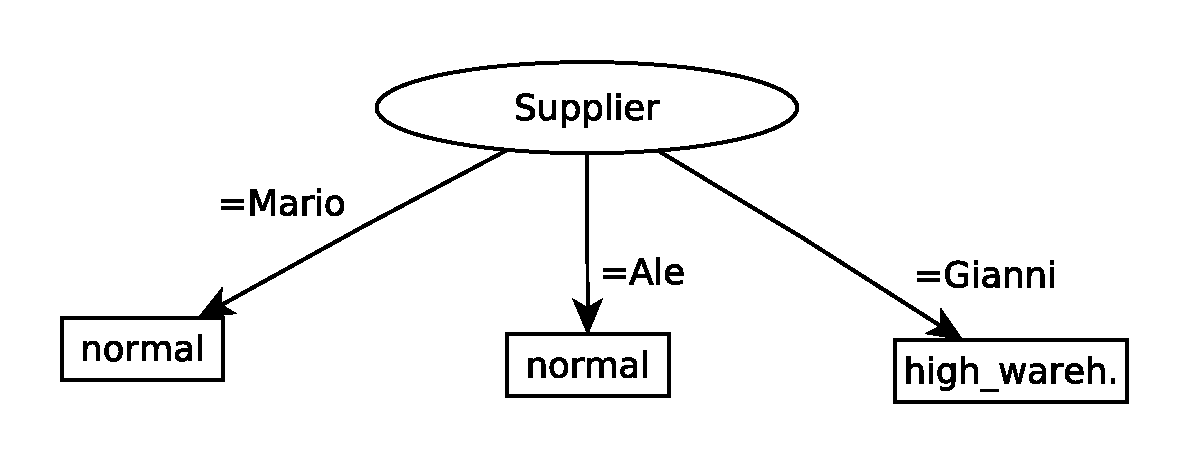
\includegraphics[width=140pt,height=80pt]
{./items/Sales_perf_tree.pdf}
\caption{decision tree}
\label{salesPerfDecTree}
\end{figure}

The decision tree shows that the syncronization time is too high, so not acceptable, for instances in which the external warehousing is done by the supplier ``Gianni''. In other general terms, the rule detected by the decision tree correlates the process performance with something regarding the warehousing. So the process efficiency dependes on the provision policy of the organization. 

\section{Implementation with ProM Framework}
In order to do experiments with some business process prototype, the approach presented in this paper has been implemented as a set of plugins that integrates the \emph{ProM6}, a process mining framework \cite{}, and \emph{Weka}, a datamining framework providing tools about classification and other techniques. 
We can divide the plugins in three classes:
\begin{itemize}
\item Plugins for managing the event log: with these plugins the goal is parsing the event log which traces the business process, extracting significant attributes and preparing the data set. There are three plugin in this class:\\
\begin{itemize}
\item \emph{Generate Instances With Conformance:} this plugin takes as input an event log and returns as output a complete data set with the target attribute as shown in figure \ref{tab:SaleData}. The data set returned respects the format needed by Weka classification tool.
\item \emph{Generate Instances With Performance}: this plugin is analogous to the previous one, but the data set generated in this case has as target attribute something characterizing the process performance as discussed in section \ref{ClassPerf}.
\item \emph{Generate Instances to Classify}: starting from an event log, with this plugin the goal is to generate a set of instances for which the conformance (or performance) result is unknown. The instances generated can be classified using an existing classification model.\\
\end{itemize}
\item Plugins for managing the classification: with these plugins the goal is to generate a classification model based on a data set and to use it for classifying unknowm records. In fact, in this class we find two plugins:\\
\begin{itemize}
\item \emph{Generate Classifier}: given a data set in which target attribute is known, this plugin uses tools provided by \emph{Weka} library to generate a classifier. In particular, the model generated is a decision tree built using $J48$ algorithm, the implementation of $C4.5$ developed by \emph{Weka}.
\item \emph{Classify Instances}: given a set of not classified instances and a classifier model, this plugin simply classify the instances according to the classifier. \\
\end{itemize}
\item Plugins managing resources: in this class we find a set of plugins useful for the serialization (and deserialization) of the resources used by the previous plugins, such as data set and classifiers. There are also some plugins allowing the visualization of these resources into \emph{ProM6} framework.
\end{itemize}


\end {document}

